

\begin{figure}[H]
  \centering
  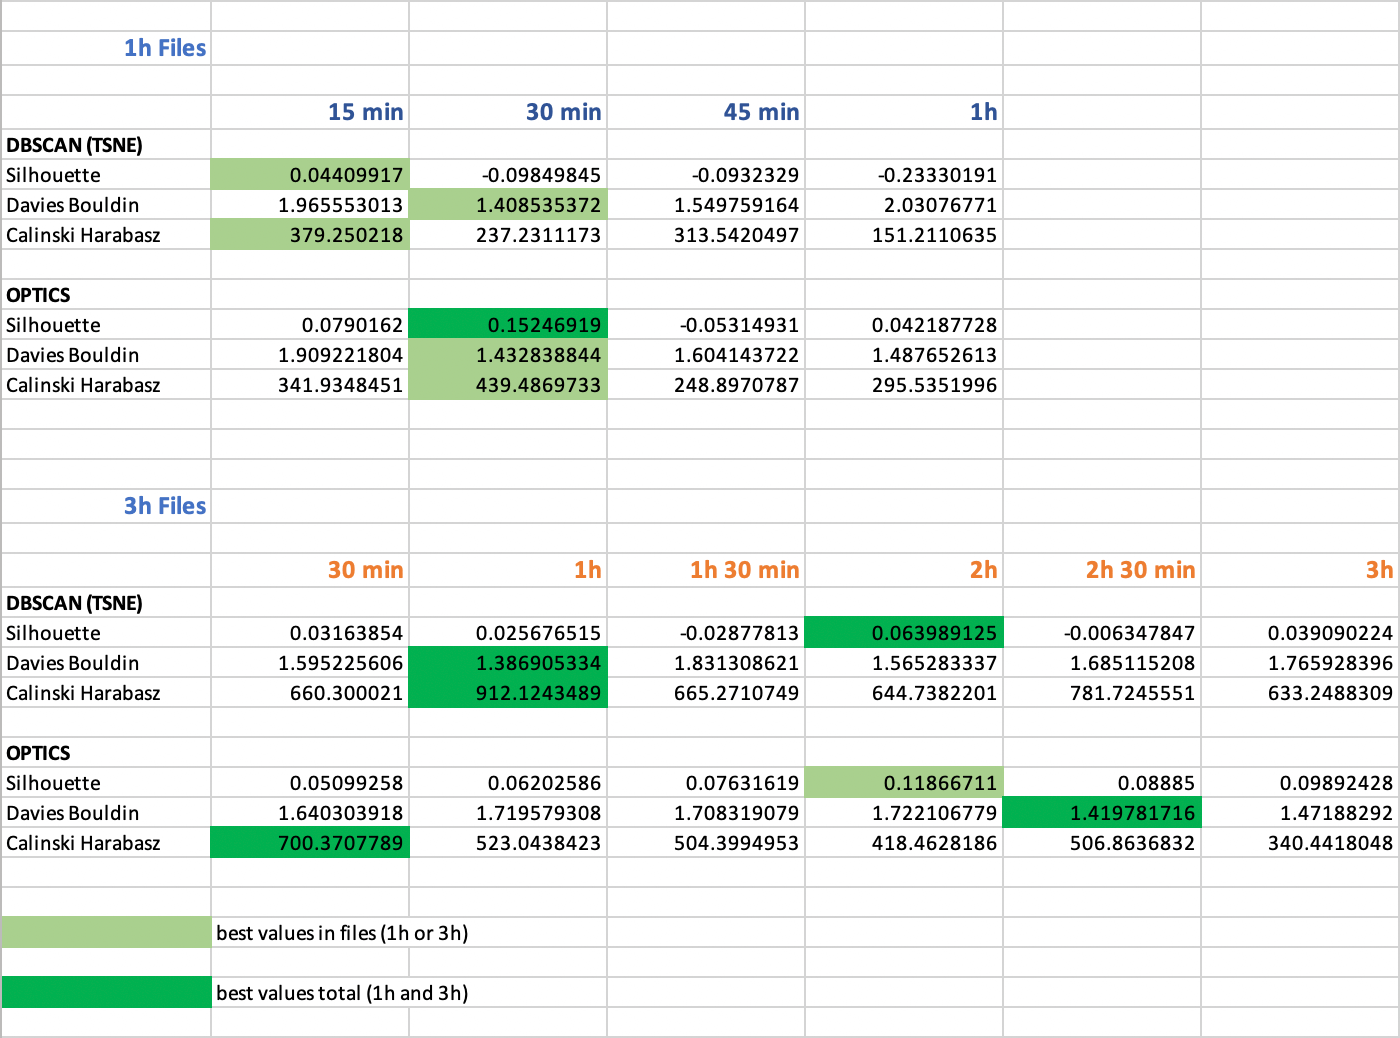
\includegraphics[width=0.8\textwidth]{./images/clusteringResults/clusteringResults1.png}
  \caption{Evaluation scores comparison from the first 1h run of t-SNE and clustering with a learning rate of 20. The lighter green highlighted values indicate the best values of that file aggregation (1h or 3h files). The dark green highlighted values illustrate the overall best values over all files (1h and 3h files).}
  \label{figure:clusteringResults1}
\end{figure}

\begin{figure}[H]
  \centering
  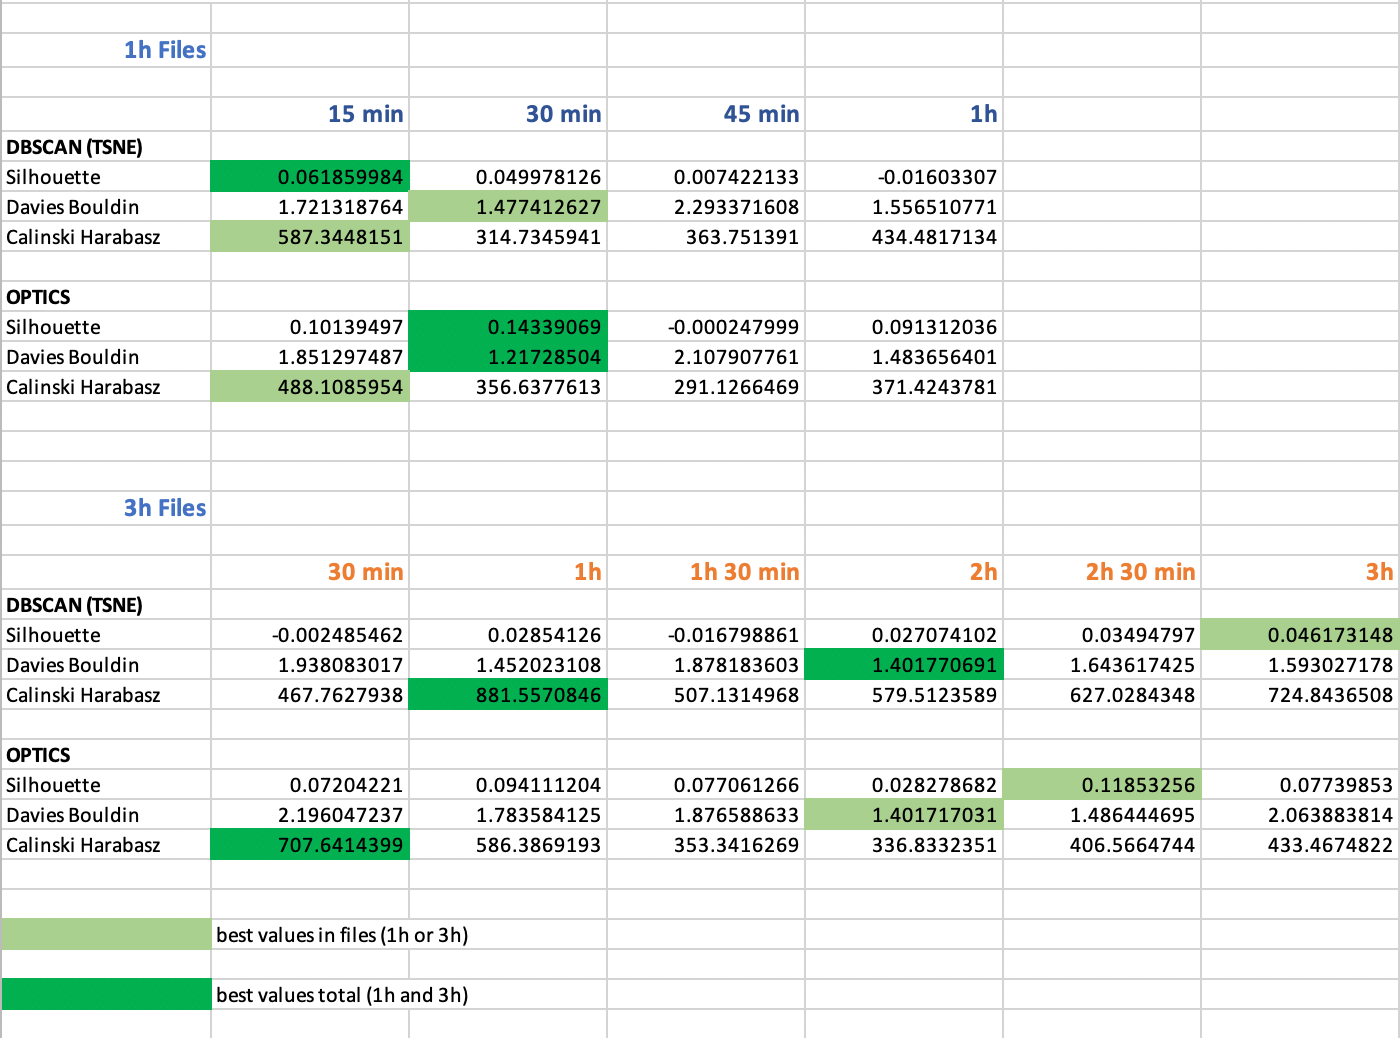
\includegraphics[width=0.8\textwidth]{./images/clusteringResults/clusteringResults2.png}
  \caption{Evaluation scores comparison from the second 1h run of t-SNE and clustering with a learning rate of 20. The lighter green highlighted values indicate the best values of that file aggregation (1h or 3h files). The dark green highlighted values illustrate the overall best values over all files (1h and 3h files).}
  \label{figure:clusteringResults2}
\end{figure}


\begin{figure}[H]
  \centering
  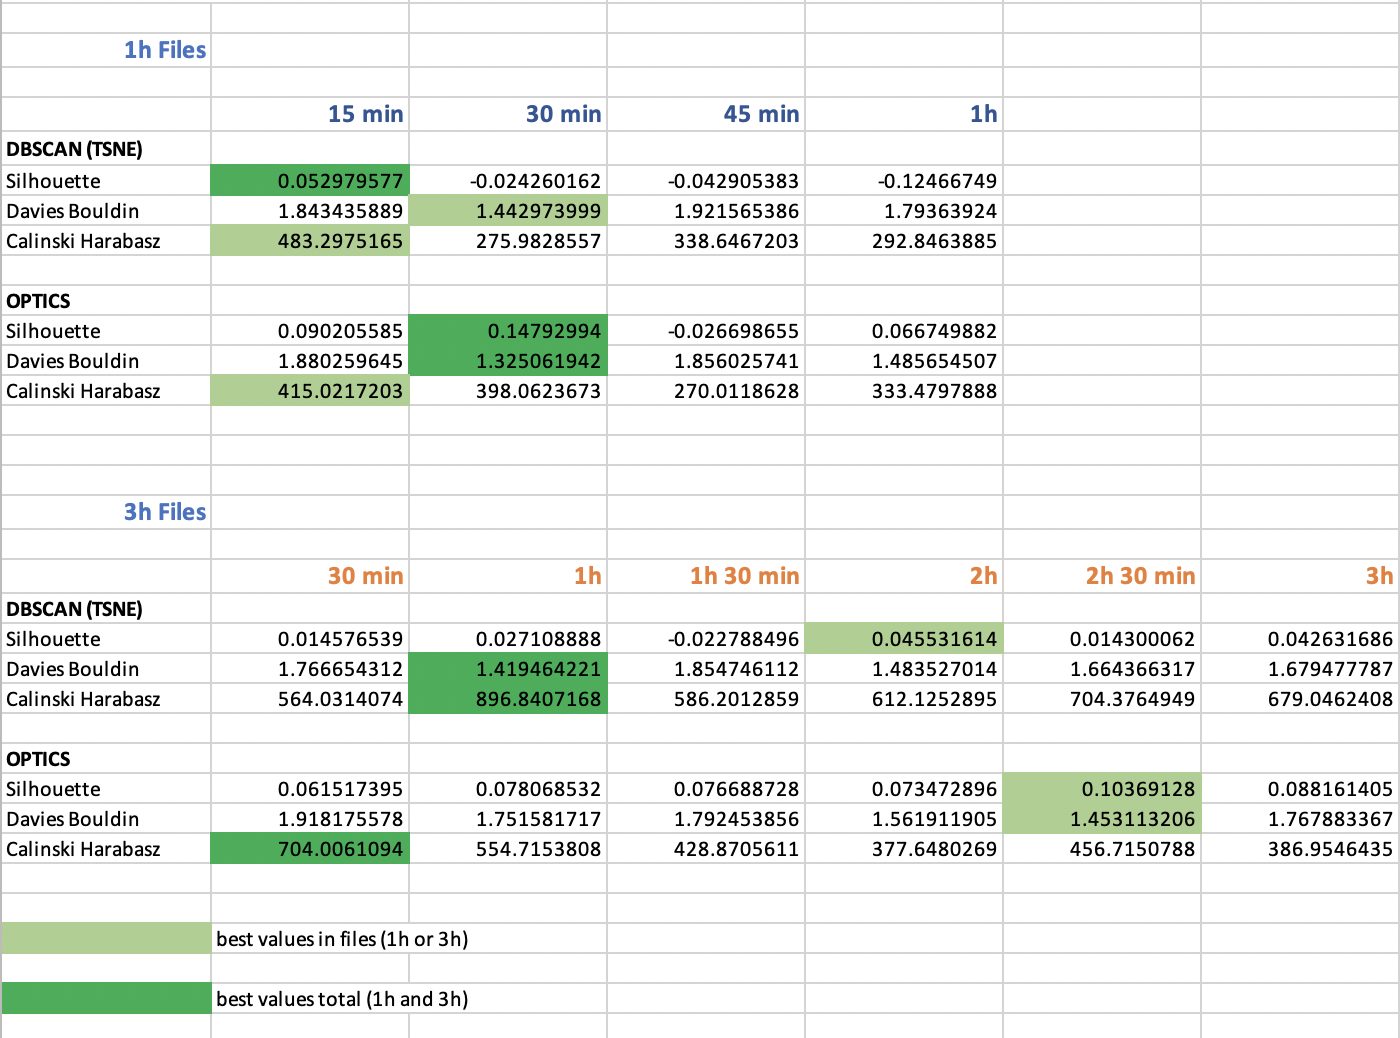
\includegraphics[width=0.8\textwidth]{./images/clusteringResults/clusteringResults3.png}
  \caption{Evaluation scores comparison averaged from figures \ref{figure:clusteringResults1} and \ref{figure:clusteringResults2}. The lighter green highlighted values indicate the best values of that file aggregation (1h or 3h files). The dark green highlighted values illustrate the overall best values over all files (1h and 3h files).}
  \label{figure:clusteringResults3}
\end{figure}

\begin{figure}[H]
  \centering
  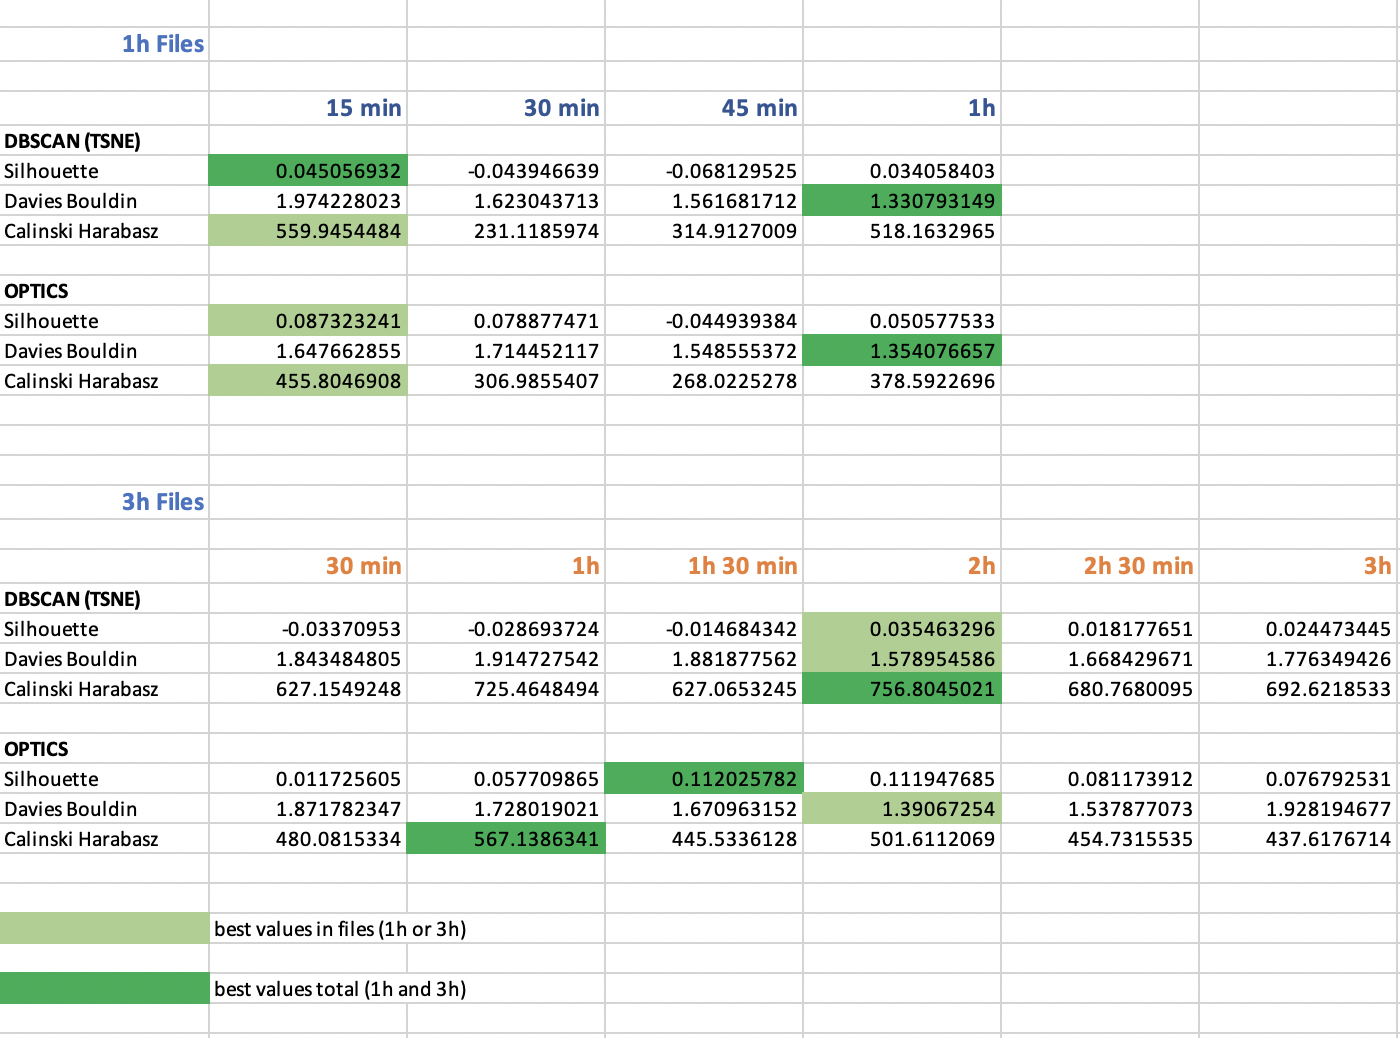
\includegraphics[width=0.8\textwidth]{./images/clusteringResults/clusteringResults4.png}
  \caption{Evaluation scores comparison averaged from 2 runs of t-SNE and clustering with a learning rate of 20. The lighter green highlighted values indicate the best values of that file aggregation (1h or 3h files). The dark green highlighted values illustrate the overall best values over all files (1h and 3h files).}
  \label{figure:clusteringResults4}
\end{figure}

\begin{figure}[H]
  \centering
  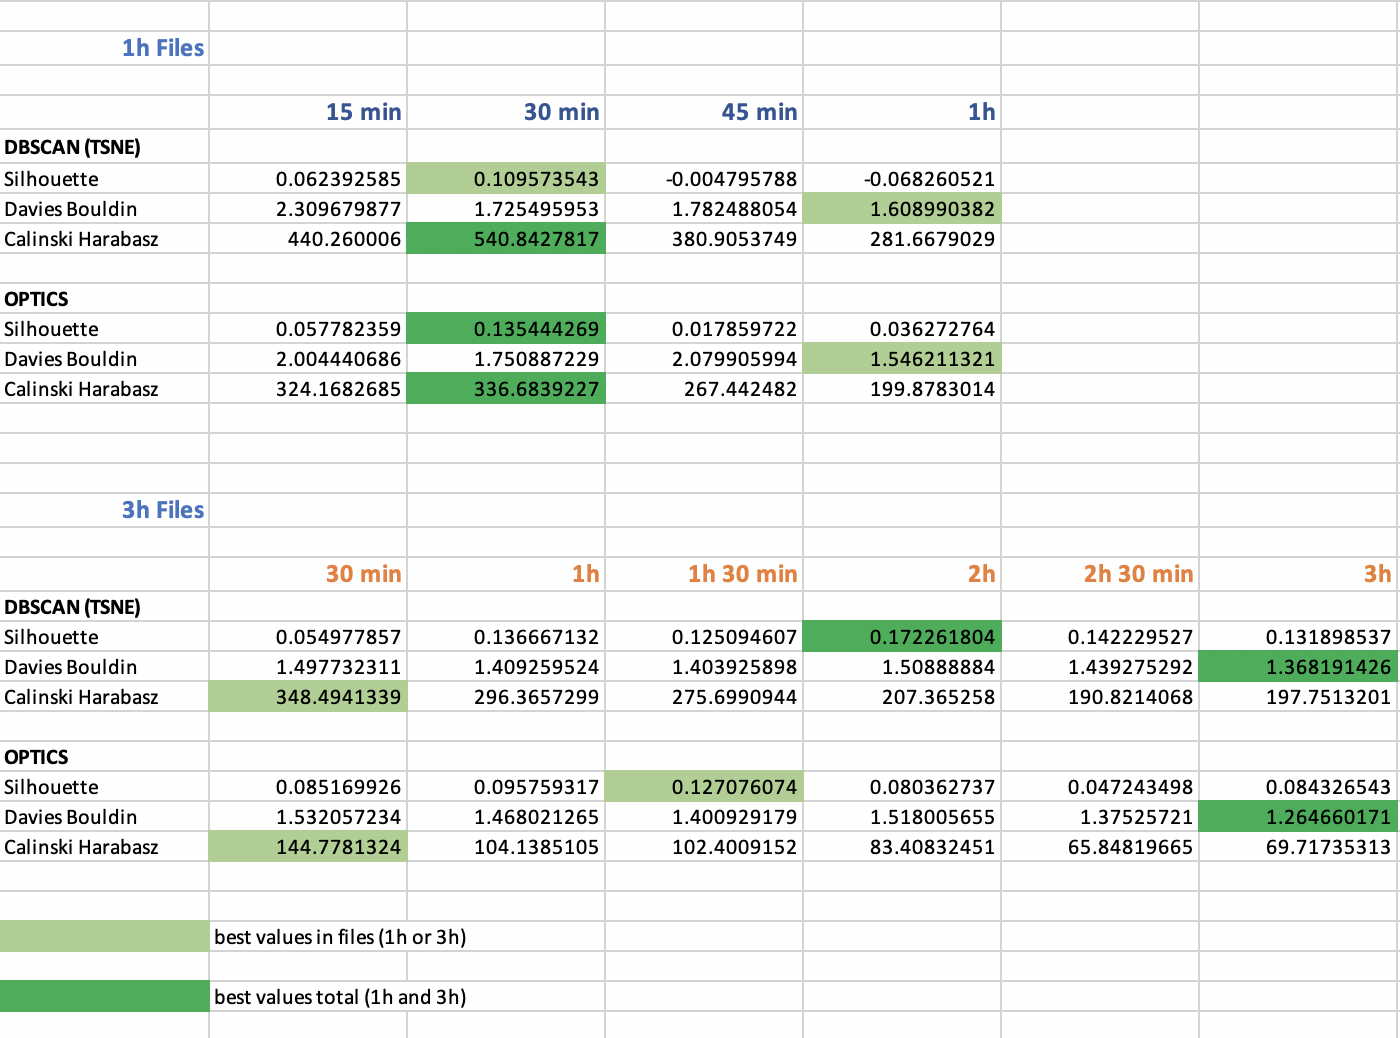
\includegraphics[width=0.8\textwidth]{./images/clusteringResults/clusteringResults5.png}
  \caption{Evaluation scores comparison averaged from 2 runs of t-SNE and clustering with a learning rate of 800. The lighter green highlighted values indicate the best values of that file aggregation (1h or 3h files). The dark green highlighted values illustrate the overall best values over all files (1h and 3h files).}
  \label{figure:clusteringResults5}
\end{figure}


\clearpage